\section{Integration Strategy}

\subsection{Entry Criteria}
For each component we state which criteria must be satisfied before starting testing. Please note that the criteria do not cover the requirements for a fully complete test, but only for starting testing.\\
SBL:
\begin{itemize}
    \item \textbf{Booking Handler:} all other SBL components are tested.
    \item \textbf{Zone Manager:} at least one between Vehicle Tracker and Special Areas Assistant is tested.
    \item \textbf{Account Manager:} none.
    \item \textbf{Payment Processor:} none.
    \item \textbf{Vehicle Tracker:} none.
    \item \textbf{Special Areas Assistant:} none.
    \item \textbf{PEJ Context:} none.
\end{itemize}
User Device Mobile App:
\begin{itemize}
    \item \textbf{Account:} none.
    \item \textbf{View:} all other UDMA components, except View Router, are tested.
    \item \textbf{View Router:} all other UDMA components, except View, are tested.
    \item \textbf{Map Wrapper:} none.
    \item \textbf{Map Explorer:} Map Wrapper is tested.
    \item \textbf{Reserved Car Viewer:} Map Wrapper is tested.
\end{itemize}
Onboard Ride Assistant App:
\begin{itemize}
    \item \textbf{Status Monitor:} none.
    \item \textbf{Map Wrapper:} none.
    \item \textbf{View:} all other ORAA components, except View Router, are tested.
    \item \textbf{View Router:} all other ORAA components, except View, are tested.
\end{itemize}
Other components:
\begin{itemize}
    \item \textbf{Client API/Accounting:} none.
    \item \textbf{Client API/Booking:} none.
    \item \textbf{Live Vehicle API:} none.
\end{itemize}
The remaining components do not need to be tested as they are provided by third parties. They will be used in testing the previously listed components that rely on them:
\begin{itemize}
    \item \textbf{Entity Framework}
    \item \textbf{Payment Processor Provider}
    \item \textbf{Mail Server}
    \item \textbf{Google Maps}
    \item \textbf{Navigator}
\end{itemize}

\subsection{Elements to be Integrated}
PEJ System is composed of three major subsystem: Service Business Logic, User Device Mobile App and Onboard Ride Assistant App.\\
The SBL provides the core functions of the service, in order to do so is is composed by the following components: Booking Handler, Zone Manager, Account Manager, Payment Processor, Vehicle Tracker, Special Areas Assistant, PEJ Context.\\
The User Device Mobile App connects to SBL via APIs, Client API/Accounting and Client API/Booking. Its components are: Account, View, View Router, Map Wrapper, Map Explorer, Reserved Car Viewer.\\
The Onboard Ride Assistant App connects to the SBL via Client API/Booking. Its components are: Status Monitor, Map Wrapper, View, View Router.\\
In order to fulfil their function the subsystems relies on the following components: Entity Framework, Live Vehicle API, Payment Processor Provider, Mail Server, Google Maps and Navigator.


\subsection{Integration Testing Strategy}
We apply a bottom-up-like testing strategy on each subsystem, in order to minimize the need for stubs and to ensure the testing phase can proceed in parallel for all three subsystems, furthermore components can be tested as soon as they are developed without needing for the entire subsystem to be completed. Since all the subsystems need to communicate one another it is not possible to apply a pure bottom-up strategy and avoid using stubs.\\
Both Client APIs and Live Vehicle API can be tested immediately using test drivers and stubs, these components are tested immediately in order to ensure no communication problem caused by API components will arise when integrating the subsystems. At the same time the testing on subsystems can starts. The PEJ Context component in SBL is the one all other components of SBL rely on to get the data they need, so its test will be carried out through testing of other components. Further components that can be initially tested are Map Wrapper in both User Device Mobile App and Onboard Ride Assistant App, since both Navigator and Google Maps are provided by third parties and are already available at the beginning of the test phase. Other components that can be tested immediately are Status Monitor in ORAA and Account in UDMA.\\
Further details about the rationale of this strategy can be found in the next section of the document, along with all the explanation about how to proceed for the integration testing.


%INTEGRATION
\subsection{Sequence of Component Integration}
Components outside the subsystems that must be tested are Client API/Accounting, ClientAPI/Booking, Live Vehicle API. These three are tested using test drivers and stubs.


\subsubsection{Software Integration Sequence}

%ORAA
\paragraph{Onboard Ride Assistant App subsystem}
The first components to be tested are Map Wrapper and Status Monitor, since the first requires only the IMapProvider interface provided by Navigator, while the second requires a stub for the ClientAPI/Booking too. See \textit{Figure 1}.
\begin{figure}[h!]
    \centering
    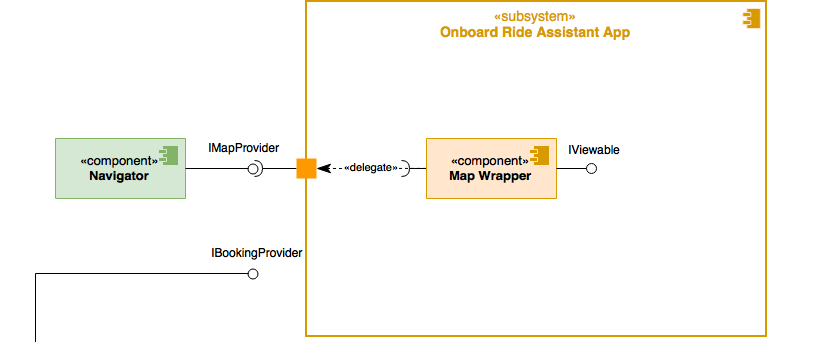
\includegraphics[scale=0.4]{{Figures/Integration/Integration1Car.png}}
    \caption{ORAA Phase One}
    \label{fig:ORAA1}
    %TEXT
\end{figure}
\\Last components of the Onboard Ride Assistant App to be tested are View and View Router, whose testing will be carried out ensuring that all possible navigation paths established in the UX Diagram contained in the Design Document are possible, and the View always provide the right information with respect to UX Diagram and the mockups in RASD. See \textit{Figure 2}.
\begin{figure}[h!]
    \centering
    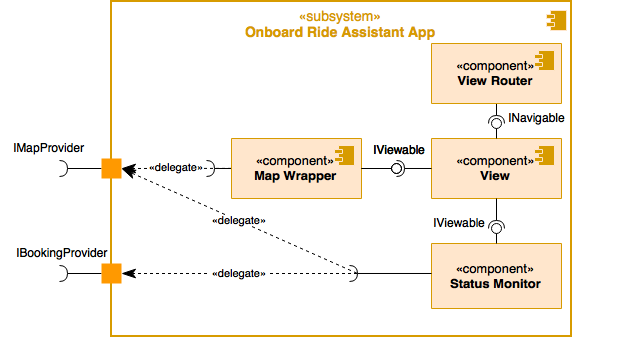
\includegraphics[scale=0.4]{{Figures/Integration/Integration2Car.png}}
    \caption{ORAA Phase Two}
    \label{fig:ORAA2}
    %TEXT
\end{figure}



\newpage
%SBL
\paragraph{Service Business Logic subsystem}
\begin{comment}
As said before, PEJ Context is the first component of SBL to be tested. See \textit{Figure 3}.
\begin{figure}[h!]
    \centering
    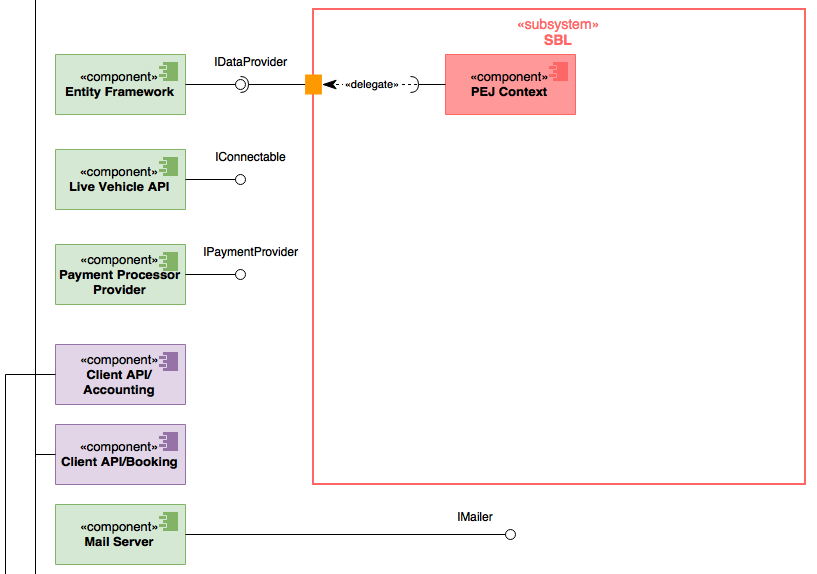
\includegraphics[scale=0.3]{{Figures/Integration/Integration1SBL.png}}
    \caption{SBL phase one}
    \label{fig:SBL1}
    %TEXT
\end{figure}
\end{comment}
Four components can be tested at the same time: Special Areas Assistant and Vehicle Tracker, which require a test driver since Zone Manager is not tested, and also a stub of Live Vehicle API for Vehicle Tracker; Payment Processor and Account Manager, which require a driver since Booking Handler is not tested. Furthermore Account Manager will use a test driver of ClientAPI/Accounting, while the IMAiler interface can be used for mail related functions. See \textit{Figure 3}.

%FOLLOWING COMMAND ADDED JUST TO CONVINCE LATEX TO DO WHAT I WANT, NOT WHAT IT WANTS
\newpage

\begin{figure}[h!]
    \centering
    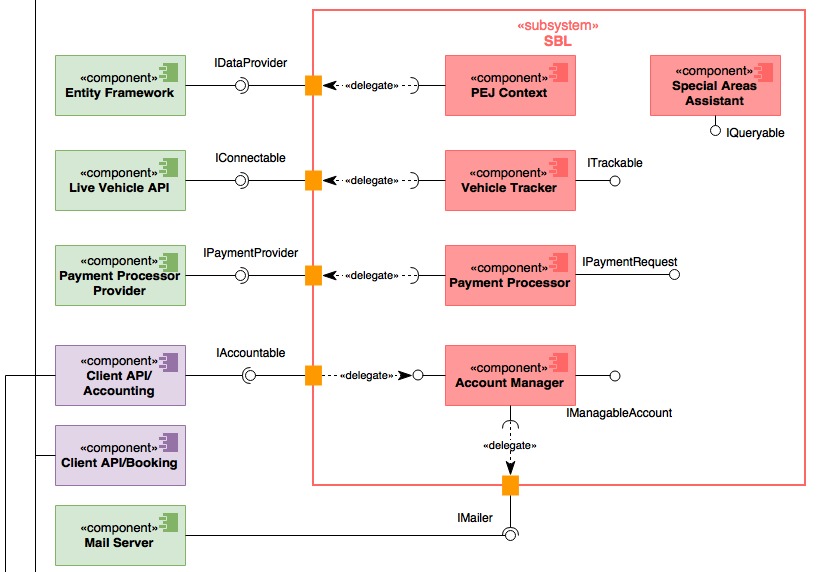
\includegraphics[scale=0.3]{{Figures/Integration/Integration2SBL.png}}
    \caption{SBL Phase One}
    \label{fig:SBL2}
    %TEXT
\end{figure}
Zone Manager is being tested; except for Booking Handler, all components are now tested; this way Zone Manager doesn't need any stub and can be tested using just one test driver instead of the actual Booking Handler. See \textit{Figure 4}.
\begin{figure}[h!]
    \centering
    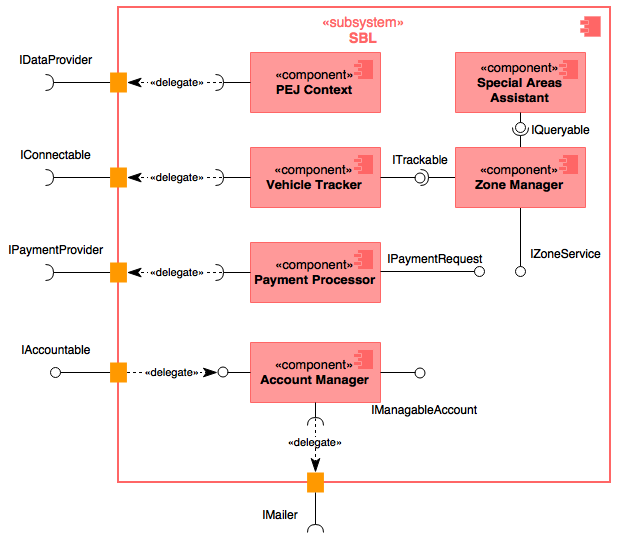
\includegraphics[scale=0.3]{{Figures/Integration/Integration3SBL.png}}
    \caption{SBL Phase Two}
    \label{fig:SBL3}
    %TEXT
\end{figure}
\\All other components are tested, so now Booking Manager can be tested without the need for any stub or driver. See \textit{Figure 5}.
\begin{figure}[h!]
    \centering
    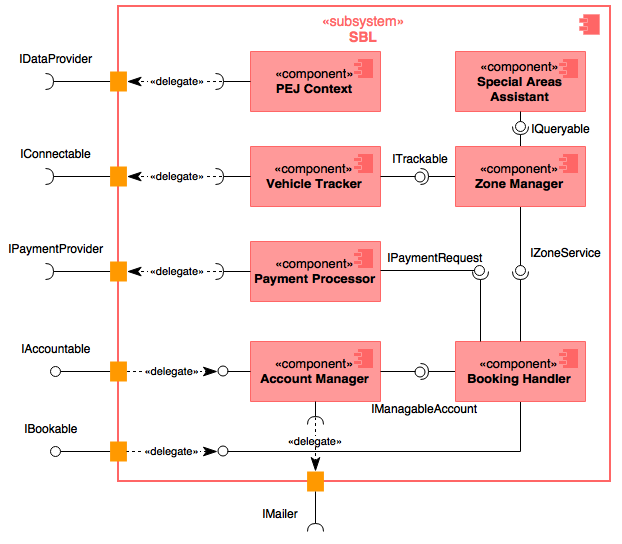
\includegraphics[scale=0.3]{{Figures/Integration/Integration4SBL.png}}
    \caption{SBL Phase Three}
    \label{fig:SBL4}
    %TEXT
\end{figure}

%The following command adds a blank page
\newcommand\blankpage{%
    \null
    \thispagestyle{empty}%
    \addtocounter{page}{-1}%
    \newpage}
\newpage


%UDMA
\paragraph{User Device Mobile App subsystem}
First components to the tested are Map Wrapper and Account. The first relies on Google Maps to get the data it needs, a test driver is used for testing; while Account requires also a stub in addition to the test drive. See \textit{Figure 6}.
\begin{figure}[h!]
    \centering
    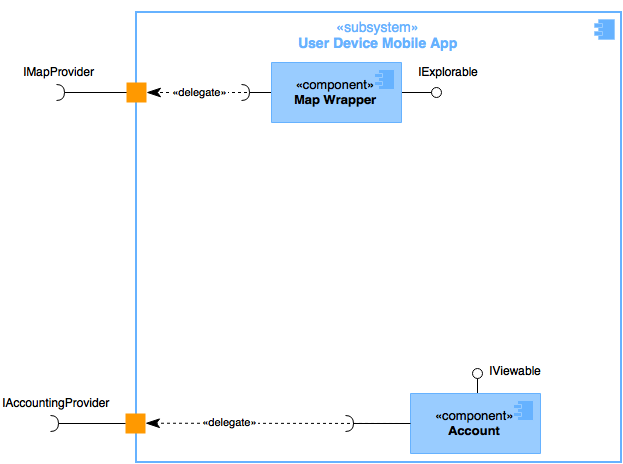
\includegraphics[scale=0.3]{{Figures/Integration/Integration1Mobile.png}}
    \caption{UDMA Phase One}
    \label{fig:UDMA1}
    %TEXT
\end{figure}
\\Next are Map Explorer and Reserved Car Viewer. These components are tested using the actual Map Wrapper component and the data provided by a stub of CLientAPI/Booking. See \textit{Figure 7}.
%FOLLOWING COMMAND ADDED JUST TO CONVINCE LATEX TO DO WHAT I WANT, NOT WHAT IT WANTS    
\newpage
\begin{figure}[h!]
    \centering
    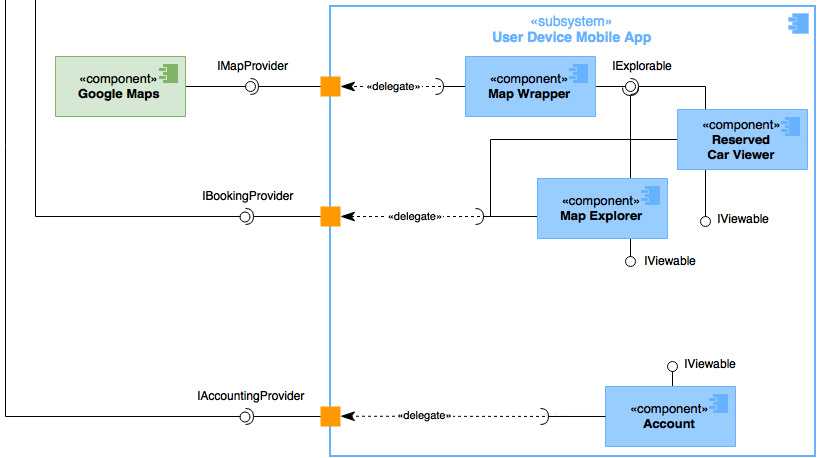
\includegraphics[scale=0.3]{{Figures/Integration/Integration2Mobile.png}}
    \caption{UDMA phase two}
    \label{fig:UDMA2}
    %TEXT
\end{figure}
Lastly View and View Router, whose testing will be carried out ensuring that all possible navigation paths established in the UX Diagram contained in the Design Document are possible, and the View always provide the right information with respect to UX Diagram and the mockups in RASD. See \textit{Figure 8}.
\begin{figure}[h!]
    \centering
    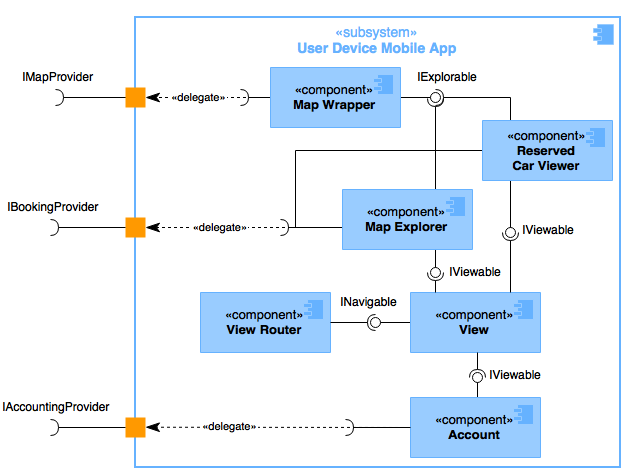
\includegraphics[scale=0.3]{{Figures/Integration/Integration3Mobile.png}}
    \caption{UDMA Phase Three}
    \label{fig:UDMA3}
    %TEXT
\end{figure}


\newpage
\subsubsection{Subsystem Integration Sequence}
After the single subsystems have been tested it is possible to integrate them. It is likely that, due to its complexity, SBL will be the last subsystem to be fully tested, which means that by the time it is tested the other two subsystems will be already tested. Therefore the integration sequence can start either from ORAA or from UDMA by integrating them with ClientAPIs, both ClientAPI/Booking and ClientAPI/Accounting where needed. After that, SBL is integrated with Live Vehicle API and ClientAPIs. The final result can be seen in \textit{Figure 9} with all third parties components already added.
\begin{figure}[h!]
    \centering
    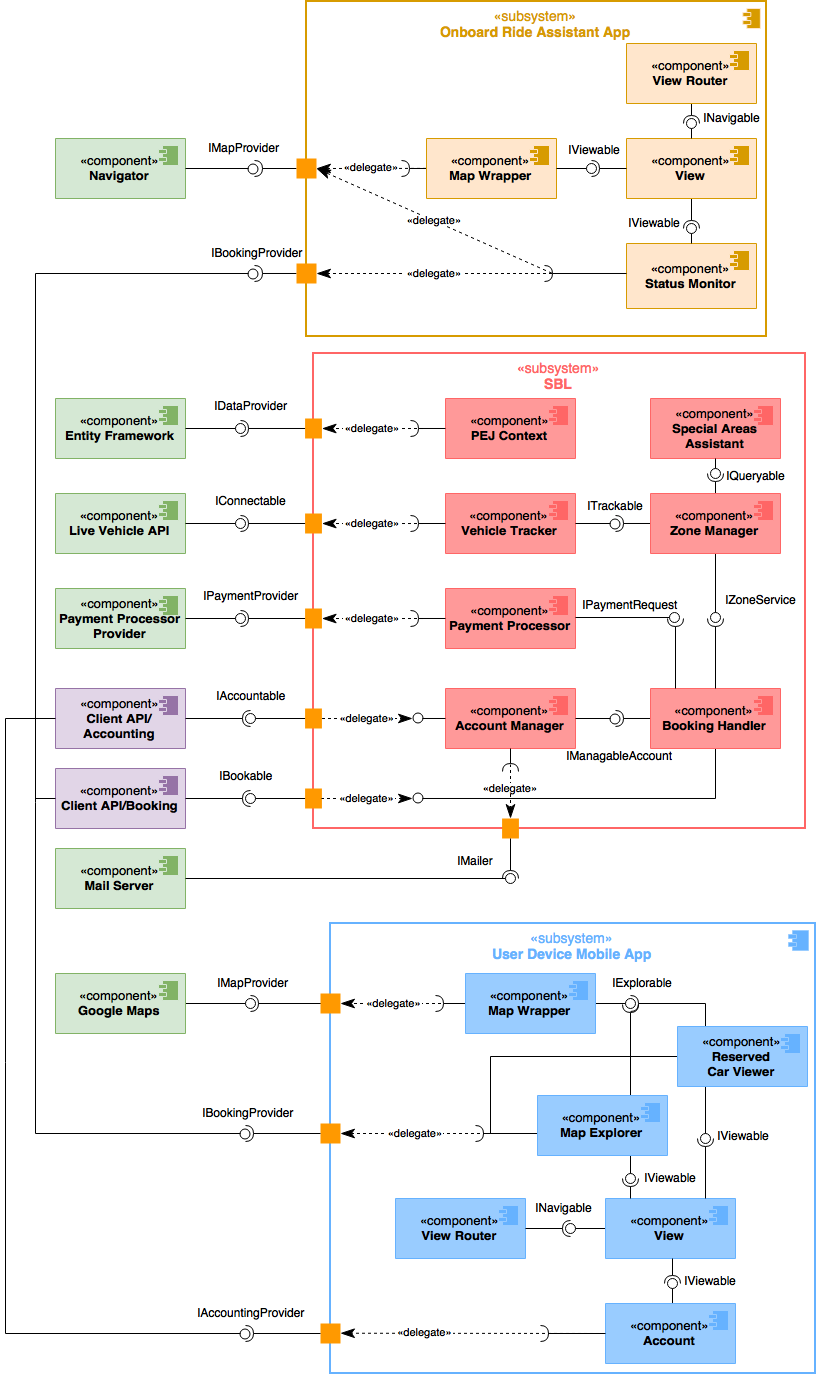
\includegraphics[scale=0.3]{{Figures/Integration/IntegrationFULL.png}}
    \caption{Integrated Subsystems}
    \label{fig:FULL}
    %TEXT
\end{figure}